\section{Results using ROS Navigation}
Much of this work is motivated by our experiences with the ROS navigation stack \cite{marder:office}. Initially, it did not have a way to directly input non-lethal obstacles. One could only input lethal obstacles, and have a small buffer of non-lethal obstacles surround it, which made it difficult to model people's personal space. As a result, we created a branch of the navigation stack that allowed for arbitrary changes to be made to the costmap. Typical parameters for the global costmap involve a grid resolution of 5 centimeters and a planning constant of $P=50$. Amplitudes can range from $[0, 254]$ and variance was typically set between $0$ and $2$. The robot was command to move from $(-3[m], 0)$ to $(+3[m], 0)$. The costmap data is then passed into a modified wavefront planner that performs interpolated gradient descent to determine a smooth path, one not constrained by the shape of the grid. The robot used to perform the sensing of the environment was Willow Garage's PR2. For these experiments, only data from the base planar laser range finder. 

The biggest question that these experiments intended to figure out was whether the same relations between parameters that we observed in the simple 4-connected grid would hold up in this less restricted environment. We found that the same principles apply, although the constants have different values. Since costmaps and the discretized paths they produce are all approximations of the same continuous space, it is logical that the different grid connectivities would have similar results; however, it is nice to have the technical confirmation to back up the ideas. Not only is the solution more general, but it has the added benefit that the resulting smoother paths are more legible to people observing the robot. 

\begin{figure*}[b]
\centering
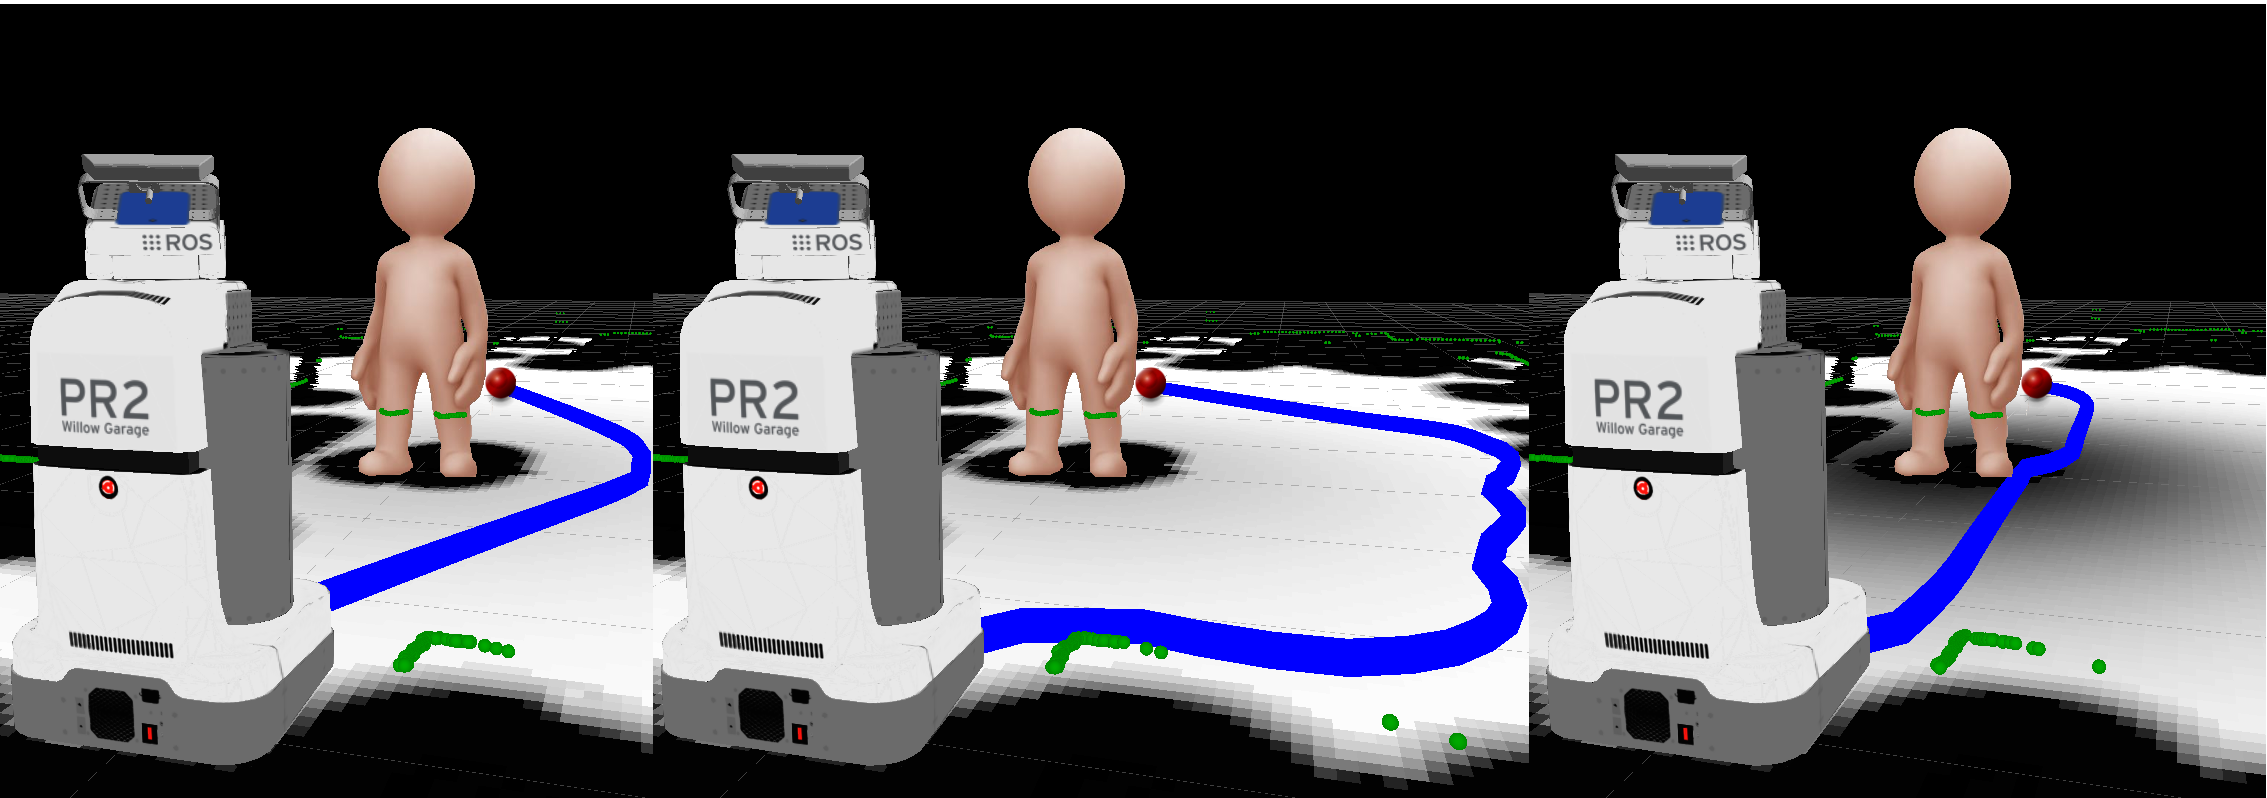
\includegraphics[width=\textwidth]{graphix/PR2-A.png}
\caption{Results using ROS Navigation, $\sigma=1.75$, and left to right, $P/A = \{3/3, 3/60$ and $3/235\}$}
\label{fig:A}
\end{figure*}

We already saw the resulting paths when $A=0$ and when $P/A = 3/3$ and $\sigma=1.75$. In Figure \ref{fig:A}, you can see three different values of $A$ as they increase, they first expand $\yhat$, but then when $A$ is very large, it contracts back down to $\yhat\approx0$. In separate trials, we also observed $\yhat$ being reduced to near 0 as $\sigma$ increased to very large values. 


\begin{figure*}[b]
\centering
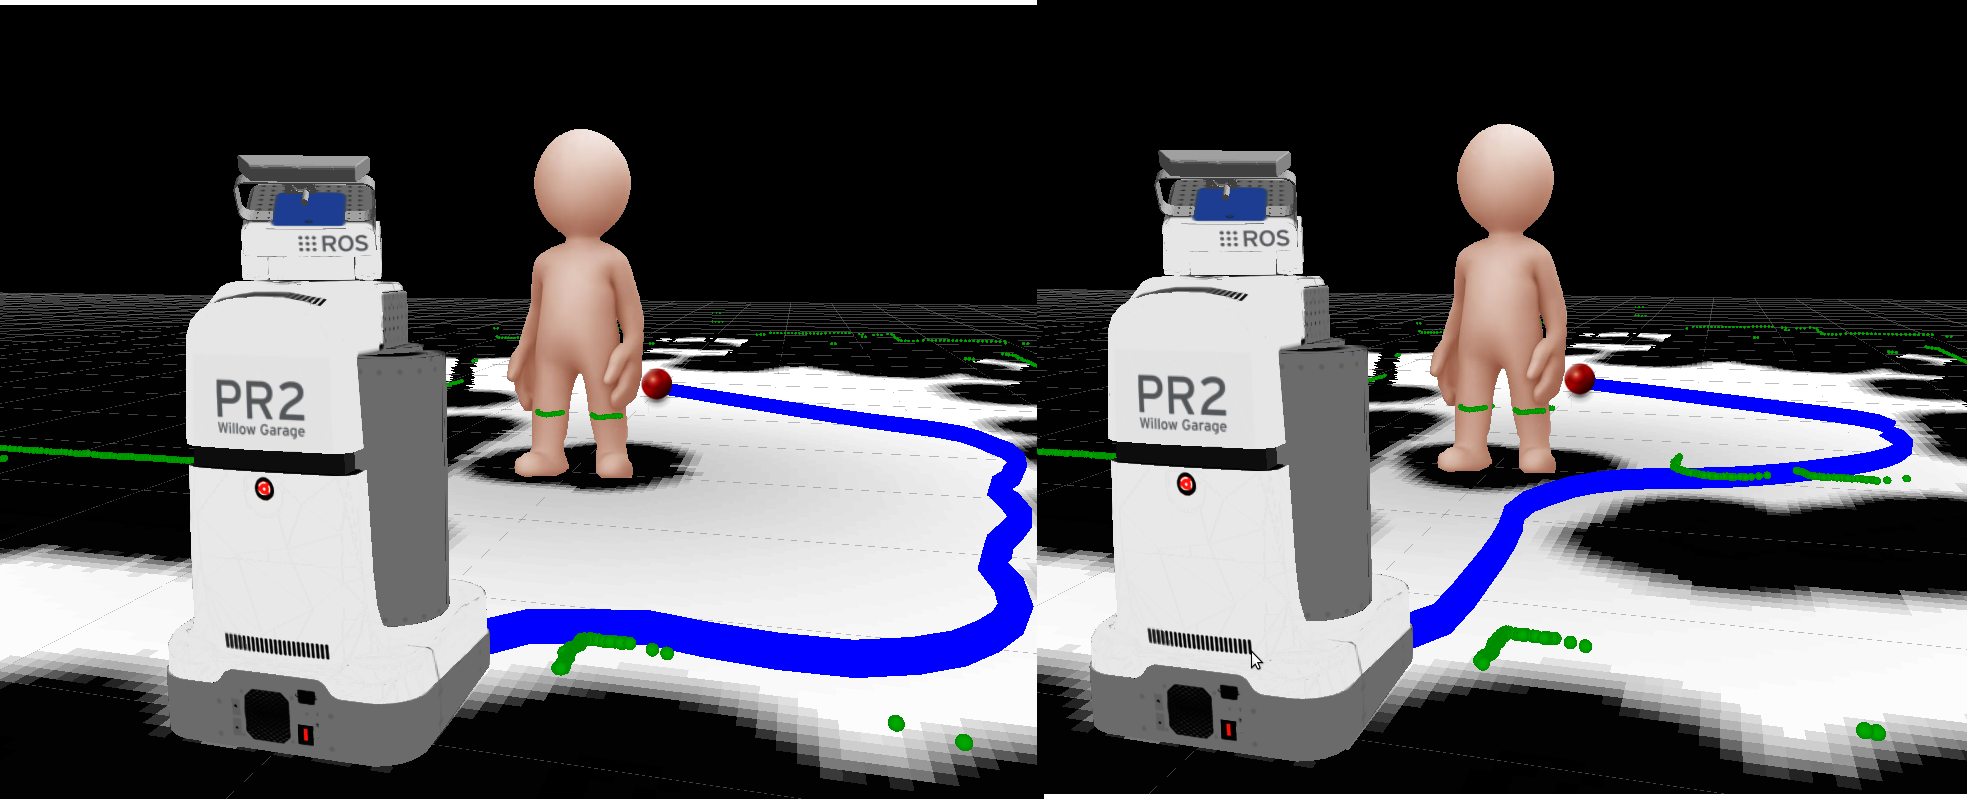
\includegraphics[width=.8\textwidth]{graphix/obstacle.png}
\caption{Results using ROS Navigation, with an obstacle and without}
\label{fig:o}
\end{figure*}

We can also see in Figure \ref{fig:o} one of the benefits of having non-lethal obstacles as opposed to lethal, in that when an obstacle is introduced into the scene, the path can go into the non-lethal area if it has to. 


